\documentclass[11pt,a4paper]{article}
\usepackage[utf8]{inputenc}
\usepackage[T1]{fontenc}
\usepackage{amsthm} %numéroter les questions
\usepackage[frenchb]{babel}
\usepackage{datetime}
\usepackage{xspace} % typographie IN
\usepackage{hyperref}% hyperliens
\usepackage[all]{hypcap} %lien pointe en haut des figures
\usepackage[french]{varioref} %voir x p y
\usepackage{fancyhdr}% en têtes
%\input cyracc.def
\usepackage[]{graphicx} %include pictures
\usepackage{pgfplots}
\usepackage[ ]{circuitikz}
\usepackage{ifthen}

\usepackage[top=1.3 in, bottom=1.3 in, left=1.3 in, right=1.3 in]{geometry} % Yeah, that's bad to play with margins
\usepackage[]{pdfpages}

\usepackage[]{attachfile}

\usepackage[many]{tcolorbox}

\newdateformat{mydate}{2016--2017}%hack pour remplacer \THEYEAR


\newboolean{corrige}
\ifx\correction\undefined
\setboolean{corrige}{false}% pas de corrigé
\else
\setboolean{corrige}{true}%corrigé
\fi

%\setboolean{corrige}{false}% pas de corrigé

\newboolean{annexes}
\setboolean{annexes}{true}%annexes
%\setboolean{annexes}{false}% pas de annexes

\definecolor{darkblue}{rgb}{0,0,0.5}

\newboolean{mos}
%\setboolean{mos}{true}%annexes
\setboolean{mos}{false}% pas de annexes

\usepackage{aeguill} %guillemets

%% fancy header & foot
\pagestyle{fancy}
%Numero du TP :
\def \labonumber {Labo \no 1 }
\lhead{[ELEC-H-310] Choucroute numérique\\ \labonumber}
\rhead{\mydate\today\\ page \thepage}
\chead{\ifthenelse{\boolean{corrige}}{Corrigé}{}}
\cfoot{}
%%

\pdfinfo{
/Author (Quentin Delhaye, Ken Hasselmann, ULB -- BEAMS)
/Title (\labonumber ELEC-H-310)
/ModDate (D:\pdfdate)
}

\hypersetup{
pdftitle={\labonumber [ELEC-H-310] Choucroute numérique},
pdfauthor={Quentin Delhaye, Ken Hasselmann, ULB -- BEAMS},
pdfsubject={}
}

\theoremstyle{definition}% questions pas en italique
\newtheorem{Q}{Question}[] % numéroter les questions [section] ou non []

\newcommand{\reponse}[1]{% pour intégrer une réponse : \reponse{texte} : sera inclus si \boolean{corrige}
	\ifthenelse {\boolean{corrige}} {\paragraph{Réponse :} \color{darkblue}   #1\color{black}} {}
 }

\newcommand{\addcontentslinenono}[4]{\addtocontents{#1}{\protect\contentsline{#2}{#3}{#4}{}}}

\date{\vspace{-1.7cm}\mydate\today}
\title{\vspace{-2cm} \labonumber\\ Électronique numérique [ELEC-H-310]\\Introduction aux dsPIC\ifthenelse{\boolean{corrige}}{~\\Corrigé}{}}

%\author{\vspace{-1cm}}%\textsc{Yannick Allard}}

\setlength{\parskip}{0.2cm plus2mm minus1mm} %espacement entre §
\setlength{\parindent}{0pt}

\begin{document}
\pagestyle{empty}
\maketitle
% \vspace*{-1cm}
\section*{But de la manipulation}
L’objectif de cette manipulation est d’introduire un microcontrôleur d’une famille couramment utilisée~: les PIC de Microchip.
Quelques systèmes simples basés sur des entrées-sorties seront réalisés.
En parallèle, ce premier labo vous aidera à vous familiariser avec le langage C
Par la suite, nous verrons comment réaliser un programme régi par le temps.

% \section*{Prérequis}
% Il est encore conseillé de lire les sections 1 à 5 du complément «~Programmation d’une carte à microcontrôleur~».

\section*{Objectifs}
À la fin de ce laboratoire vous devez être capables~:
\begin{itemize}
\item De réaliser un programme simple pour microcontrôleur.
\item D’expliquer la notion d’entrées-sorties ainsi que la sortance.
\item De faire intervenir des éléments asynchrones dans votre programme par le biais de
timers.
\end{itemize}
\newpage{}


\section{Introduction}
Au long des six laboratoires qui illustrent le cours, vous serez amenés à utiliser une carte à microcontrôleur.
En plus de la programmer, vous devrez comprendre le fonctionnement de ses différents périphériques et l’interfacer avec le monde extérieur.

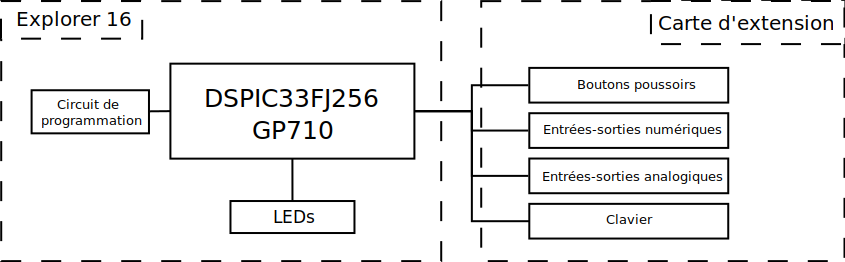
\includegraphics[width=\textwidth]{pic33}

Ce premier laboratoire a pour but de vous faire prendre en main la carte et d’utiliser quelques périphériques de base. Vous apprendrez à interagir de manière simple avec le microcontrôleur de la carte.

Le fonctionnement de la carte ainsi que du dsPIC est expliqué dans le complément «~Programmation d’une carte à microcontrôleur~». 
Pour les deux premiers labos, il vous est conseillé d’utiliser en particulier la section 4 «~Première prise en main~».


\section{Programme basique~: utilisation des entrées-sorties}
Votre premier programme consistera en l’interfaçage de deux types d’entrées-sorties~: les boutons poussoirs et les LEDS.
Le cahier des charges est simple~: on désire que la LED branchée à la borne RA0 s’allume lorsque l’on appuie sur un bouton au choix, et s’éteigne lorsqu’on le relâche.

\begin{itemize}
	\item Localisez les différents périphériques présents sur la carte fournie et cités dans le complément «~Programmation d’une carte à microcontrôleur~» (LEDs, boutons poussoirs, potentiomètre, sortie analogique connectée à l’ampli de puissance, etc.).
	\item À l’aide du complément réalisez un programme répondant au cahier des charges. Pour ce faire, et à l’aide du programme d’exemple fourni.
	\begin{itemize}
		\item Localisez la boucle while(1).
		Cette boucle sans fin contient les routines du programme qui doive tourner en continu, alors que le code situé avant la boucle n’est exécuté qu’une seule fois et sert essentiellement à configurer les périphériques et à définir les variables.
		\item Configurez les registres TRIS  des pattes d’entrée-sortie afin d’en choisir la direction (entrée OU sortie).
		\item Écrivez le corps de votre programme.
		\item Compilez et chargez le code sur la carte à $\mu$C, et vérifiez son fonctionnement.
	\end{itemize}
\end{itemize}

Après coup, on décide de plutôt utiliser une LED ultrabrillante consommant 20~mA sous 3,2~V.
Celle-ci n’étant pas présente sur la carte, vous devrez la connecter à une des bornes de la carte d’extension (voir annexe pour plus de détail).

% \par{\textbf{Rappel sur l'utilisation d'une diode.}}
% Une diode possède deux bornes~: l'anode (borne positive) et la cathode (borne négative).
% Une diode classique devant être polarisée positivement afin de laisser circuler le courant, l'anode doit être connectée à la source de tension ($\mu$C ou buffer).
% De plus, afin de limiter le courant circulant dans la diode, une résistance doit être connectée à l'anode.

\tcboxfit[height=7cm,title={Rappel sur l'utilisation d'une diode.},
  before=\noindent]{%
  Une diode possède deux bornes~: l'anode (borne positive) et la cathode (borne négative).
  Une diode classique devant être polarisée positivement afin de laisser circuler le courant, l'anode doit être connectée à la source de tension ($\mu$C ou buffer).
  De plus, afin de limiter le courant circulant dans la diode, une résistance doit être connectée à l'anode.

  \begin{center}
  	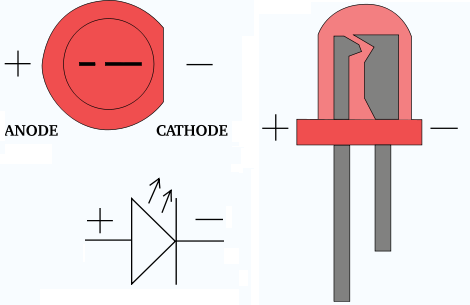
\includegraphics[width=5cm]{diagrammeLED.png}
  \end{center}

  }


\begin{itemize}
	\item Pourquoi une connexion directe entre le dsPIC et la LED ne fonctionne-t-elle pas~?
	Faites le lien avec la notion de sortance statique.
	\reponse{
		Si l'on branche directement la LED sur la sortie de la carte, elle ne s'allume qu'avec une très faible intensité.
		La carte n'est tout simplement pas capable de sortir suffisament de courant pour la LED.
	}
	\item Expliquez en quoi l’utilisation d’un circuit du type \textit{buffer} résout le problème.
	Tracez le nouveau schéma-bloc de votre système.
	\reponse{
		L'utilisation d'un buffer permet de propager la commande du microcontrôleur tout en fournissant plus de courant à la LED.
	}
\end{itemize}

Nous allons utiliser un circuit buffer 74ACT244 dont la notice est fournie en annexe.

% \begin{itemize}
% 	\item Vérifiez que ce circuit respecte bien les normes TTL 5~V.
% 	\reponse{
% 		\begin{center}
% 			\begin{tabular}{cl}
% 			 & TTL (5~V) \\ \hline
% 			 $V_{OH}$ & 2.4 V \\
% 			 $V_{iH}$ & 2.0 V \\
% 			 $V_{iL}$ & 0.8 V \\
% 			 $V_{OL}$ & 0.5 V \\
% 			\end{tabular}
% 		\end{center}
% 		~\newline{}

% 		Dans notre montage, l'entrée à l'état haut est à 3.3~V et la basse à 0~V (imposés par la carte).
% 		Étant donné que ces valeurs sont resectivement plus haute que $V_{iH}$ et plus basse que $V_{iL}$ en TTL 5~V, la norme est respectée.
% 	}
% 	\item Réalisez un montage sur protoboard permettant d’allumer la LED.
% 	N’oubliez pas de dimensionner la résistance de limitation du courant dans la diode.
% 	Alimentez le buffer en 0~V/5~V
% 	\item Modifiez votre programme pour qu’une pression sur le bouton allume désormais la LED ultra-brillante externe au lieu de celles présentes sur la carte.
% \end{itemize}



\section{Utilisation du timer}
On vous demande de faire clignoter des LEDs à une fréquence donnée.
Pour ce faire, vous aurez besoin d’utiliser un timer.
Ce périphérique intègre un registre de 16 bits s’incrémentant à chaque coup d’horloge.
Lorsque la valeur de ce registre atteint celle écrite dans le registre de période (PR1 pour le timer 1, PR2 pour le timer 2, etc.), le compteur retourne à zéro et recommence à s’incrémenter.
Dans le même temps, un bit spécifique nommé flag passe à ‘1’ pour prévenir du débordement (cf. guide de programmation).
Dans un premier temps, vous allez écrire un programme permettant de faire clignoter la LED à une fréquence de 10~kHz.

\begin{itemize}
	\item Quelle valeur doit contenir le registre de période PR du timer pour que ce dernier déborde à la bonne fréquence~?
	Quelle est la période maximale du timer~? Pour rappel, le processeur exécute des instructions au rythme de 40~MHz.
	\reponse{
		Si l'on veut que la LED clignotte à une fréquence de 10~KHz, il faut que l'état de la pin sur laquelle elle est connectée change d'état à une fréquence de 20~KHz.
		Ces 20~KHz correspondent à une période de 2000 instructions pour le timer.
		La période maximale de ce timer (sur 16 bits) est de $\frac{2^{16}-1}{40\cdot10^6} = 1638 \mu s$.
		En utilisant un \textit{prescaler} de 256, cette période peut monter jusqu'à $0,419 s$.
	}
	\item Vérifiez que l’appel à la fonction \texttt{clav2LCD} est bien mis en commentaire.
	\item Ajoutez à votre code les lignes nécessaires à la configuration et au lancement d’un timer (au choix).
	\item Dans la boucle principale de votre programme~:
	\begin{itemize}
		\item Vérifiez par polling si votre timer est arrivé à son terme (ie. Si le bit TxIF est passé à ‘1’).
		\item Écrivez une routine permettant de faire commuter la patte d’I/O RC1 à la fréquence de débordement.
		Cette routine ne peut pas être bloquante~: on doit par exemple pouvoir continuer à allumer la LED ultrabrillante à tout moment en appuyant sur un bouton.
		\item N’oubliez pas de remettre à zéro le bit TxIF dans votre routine.
	\end{itemize}
	\item Vérifiez à l’oscilloscope que la fréquence est bien celle attendue.
	\item Modifiez le programme de sorte à ce que la période soit maintenant de 500~ms, et programmez le clignotement des LEDs.
	\reponse{
		Étant donné que la période de changement d'état est de 250~ms, on peut encore utiliser un timer sur 16 bit en le couplant à un \textit{prescaler} de 256.
	}
\end{itemize}





\end{document}
